\documentclass{article}

\usepackage{fancyhdr}
\usepackage{extramarks}
\usepackage{amsmath}
\usepackage{amsthm}
\usepackage{amsfonts}
\usepackage{tikz}
\usepackage[plain]{algorithm}
\usepackage{algpseudocode}
\usepackage{graphicx}
\usepackage{gensymb}
\usepackage{calc}
\usepackage[framed,numbered,autolinebreaks,useliterate]{mcode}
\usepackage{listings}
\usepackage{empheq}
\usepackage{enumitem}
\usepackage[font=footnotesize]{caption}
\usepackage{subcaption}
\usepackage{lipsum}
\usepackage[export]{adjustbox}

\graphicspath{{./images/}}

\usetikzlibrary{automata,positioning}

%
% Basic Document Settings
%

\topmargin=-0.45in
\evensidemargin=0in
\oddsidemargin=0in
\textwidth=6.5in
\textheight=9.0in
\headsep=0.25in

\linespread{1.1}

\pagestyle{fancy}
\lhead{\hmwkAuthorLastNames}
\chead{\hmwkClass\ \hmwkTitle}
\rhead{\firstxmark}
\lfoot{\lastxmark}
\cfoot{\thepage}

\renewcommand\headrulewidth{0.4pt}
\renewcommand\footrulewidth{0.4pt}

\setlength\parindent{0pt}

%
% Create Problem Sections
%

\newcommand{\enterProblemHeader}[1]{
    \nobreak\extramarks{}{Problem {#1} continued on next page\ldots}\nobreak{}
    \nobreak\extramarks{{#1} (continued)}{{#1} continued on next page\ldots}\nobreak{}
}

\newcommand{\exitProblemHeader}[1]{
    \nobreak\extramarks{{#1} (continued)}{{#1} continued on next page\ldots}\nobreak{}
    % \stepcounter{#1}
    \nobreak\extramarks{{#1}}{}\nobreak{}
}

\setcounter{secnumdepth}{0}
\newcounter{partCounter}

\newcommand{\problemNumber}{0.0}

\newenvironment{homeworkProblem}[1][-1]{
    \renewcommand{\problemNumber}{{#1}}
    \section{\problemNumber}
    \setcounter{partCounter}{1}
    \enterProblemHeader{\problemNumber}
}{
    \exitProblemHeader{\problemNumber}
}

%
% Homework Details
%   - Title
%   - Class
%   - Author
%

\newcommand{\hmwkTitle}{Group Assignment\ \#2}
\newcommand{\hmwkClass}{RBE 500}
\newcommand{\hmwkAuthorName}{\textbf{Joshua Gross, Arjan Gupta, Melissa Kelly}}
\newcommand{\hmwkAuthorLastNames}{\textbf{Gross, Gupta, Kelly}}

%
% Title Page
%

\title{
    \vspace{2in}
    \textmd{\textbf{\hmwkClass\ \hmwkTitle}}\\
    \vspace{3in}
}

\author{\hmwkAuthorName}
\date{}

\renewcommand{\part}[1]{\textbf{\large Part \Alph{partCounter}}\stepcounter{partCounter}\\}

%
% Various Helper Commands
%

% Useful for algorithms
\newcommand{\alg}[1]{\textsc{\bfseries \footnotesize #1}}

% For derivatives
\newcommand{\deriv}[2]{\frac{\mathrm{d}}{\mathrm{d}#2} \left(#1\right)}

% For compact derivatives
\newcommand{\derivcomp}[2]{\frac{\mathrm{d}#1}{\mathrm{d}#2}}

% For partial derivatives
\newcommand{\pderiv}[2]{\frac{\partial}{\partial #2} \left(#1\right)}

% For compact partial derivatives
\newcommand{\pderivcomp}[2]{\frac{\partial #1}{\partial #2}}

% Integral dx
\newcommand{\dx}{\mathrm{d}x}

% Alias for the Solution section header
\newcommand{\solution}{\textbf{\large Solution}}

% Probability commands: Expectation, Variance, Covariance, Bias
\newcommand{\E}{\mathrm{E}}
\newcommand{\Var}{\mathrm{Var}}
\newcommand{\Cov}{\mathrm{Cov}}
\newcommand{\Bias}{\mathrm{Bias}}

\newlength\dlf% Define a new measure, dlf
\newcommand\alignedbox[2]{
% Argument #1 = before & if there were no box (lhs)
% Argument #2 = after & if there were no box (rhs)
&  % Alignment sign of the line
{
\settowidth\dlf{$\displaystyle #1$}  
    % The width of \dlf is the width of the lhs, with a displaystyle font
\addtolength\dlf{\fboxsep+\fboxrule}  
    % Add to it the distance to the box, and the width of the line of the box
\hspace{-\dlf}  
    % Move everything dlf units to the left, so that & #1 #2 is aligned under #1 & #2
\boxed{#1 #2}
    % Put a box around lhs and rhs
}
}

\begin{document}

\maketitle

\nobreak\extramarks{Problem 1}{}\nobreak{}

\pagebreak

\begin{homeworkProblem}[Problem 1]
    \subsection{Create ROS Package for PD Controller}
    \vspace{0.1in}
    \subsubsection{Preliminary Work with Gazebo}
    Before creating the ROS package for the PD controller we performed
    some reconnaissance.\\
    \vspace{0in}\\
    When we executed \lstinline{ros2 topic list}, we saw that the
    \lstinline{/forward_effort_controller/commands} topic was part of it.
    We then executed the following command in an attempt to move the joints.
    \begin{lstlisting}
        ros2 topic pub --once /forward_effort_controller/commands std_msgs/msg/Float64MultiArray "{data: [1, 1, 1]}"
    \end{lstlisting}
    \vspace{0.1in}
    However, this took no effect. We remember from the last group assignment (Part 1)
    that we executed a very similar command to make the joints move to a specific
    position, except in that case the topic we published to was
    \lstinline{/forward_position_controller/commands}. This gave us a hint to
    the fact that Gazebo was preferring the position controller over the
    effort controller. Upon discovering the \lstinline{controller_switch.cpp} file
    in the rrbot simulation files, we realized that we must `activate' the effort
    controller in order to use it.
    Next, we did some more discovery using terminal commands. We executed
    \begin{lstlisting}
        ros2 service list -t    
    \end{lstlisting}
    \vspace{0.1in}
    This helped us see that
    \lstinline{/controller_manager/switch_controller} was an available
    service we could use. Since we supplied the -t flag to this command,
    we could also see that \lstinline{controller_manager_msgs/srv/SwitchController}
    was the type of message we had to use. To further take note of the message
    type, we executed
    \begin{lstlisting}
        ros2 interface show controller_manager_msgs/srv/SwitchController
    \end{lstlisting}
    \vspace{0.1in}
    Here we could see that \lstinline{activate_controllers} and 
    \lstinline{deactivate_controllers}
    were parameters of the message. Now we put together our findings and
    executed the following command that we constructed.
    \begin{lstlisting}
        ros2 service call /controller_manager/switch_controller controller_manager_msgs/srv/SwitchController "{activate_controllers: ["forward_effort_controller"], deactivate_controllers: [forward_position_controller, forward_velocity_controller]}"
    \end{lstlisting}
    \vspace{0.1in}
    Upon doing this, we saw the the prismatic joint drop. This means something took
    effect. To further confirm the state of each controller, we used the following
    command,
    \begin{lstlisting}
        ros2 control list_controllers -v
    \end{lstlisting}
    \vspace{0.1in}
    Which showed that the position and velocity controllers were now inactive.
    We now tried our initial command,
    \begin{lstlisting}
        ros2 topic pub --once /forward_effort_controller/commands std_msgs/msg/Float64MultiArray "{data: [1, 1, 1]}"
    \end{lstlisting}
    \vspace{0.1in}
    Now we saw the robot in Gazebo move! The two revolute joints `spun' in an
    anti-clockwise direction in the XY plane, whereas the prismatic joint did
    not do anything. With some more experimentation we realized:
    \begin{itemize}
        \item Acceleration due to gravity, approximated in magnitude
        to $9.8 m/s^2$ was acting on the prismatic joint. Therefore, in order to
        make it move upward we needed to publish an effort with an acceleration
        of anything less than $-9.8 m/s^2$.
        \item In order to hold the prismatic joint
        in at any height, we needed to apply exactly $-9.8 m/s^2$ acceleration.
        The negative sign is a consequence of the direction of motion we have
        defined in our URDF file. 
        \item Since our
        joint masses are simply 1, we were able to publish a joint effort as simply
        $-9.8$, for example.
        \item We also realized that since there was no opposing force readily
        acting upon the revolute joints, if we executed an effort to them, that
        effort would keep pushing along the joints.
        \item In order to hold the revolute joints in a particular angle, we needed
        to specify that we are applying 0 effort. However this did not
        instantaneously stop the rotation of these joints, we noticed a
        de-acceleration effect before the joint came to a stop.
        \item As for implementing our package, this means that we will first
        need to execute a service call (by creating a client) to activate the
        right controller. As for executing efforts via the PD controller, we
        will need to account for gravity in case of the prismatic joint. 
    \end{itemize}

    \vspace{0.1in}
    \subsubsection{Preliminary Work for Controller}

    \begin{figure}[h]
        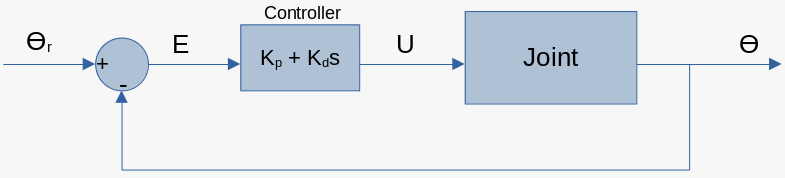
\includegraphics[scale=0.45]{closed-loop.png}
        \centering
        \caption{Standard PD controlled closed-loop system}
    \end{figure}

    Taking inspiration from how we have modeled PD controllers so far in
    this course, we can imagine the control for each joint as shown in
    Figure 1.\\
    \vspace{0in}\\
    Here, the goal position, $\theta_r$ will be received via a service call.
    Our package will must contain a service for this purpose.
    The current position $\theta$ is received via the \lstinline{/joint_states}
    topic. The error, $E$ is calculated as \(E = \theta_r - \theta\). This error
    is then with some untuned multiplier (gain) $K_p$ to obtain the first term of
    our controller.\\
    \vspace{0in}\\
    Next, we need to get the derivative of the error, $\dot{E}$, which could be
    expressed as
    \begin{align*}
        \dot{E} &= \dot{\theta_r} - \dot{\theta}\\
        \dot{E} &= 0 - \dot{\theta}\\
        \dot{E} &= - \dot{\theta} = -v
    \end{align*}
    Therefore the derivative of the error is the negative of $v$, the velocity of
    the joint. This velocity can be obtained from the \lstinline{/joint_states}
    topic or it can be approximated by looking at the position in the last `step'
    and the current step. Once we have $\dot{E}$, we use another untuned
    multiplier (gain) $K_d$ to obtain the second term of our 
    controller. Therefore, our controller is
    \[
        F = K_p E + K_d \dot{E} = K_p E - K_d v 
    \]
    Where F is the resultant effort that we need to apply to the joint.

    \vspace{0.25in}
    \subsubsection{Writing the ROS Package}
    \vspace{0.15in}
    Now we create the package just as we've done in our past assignments of this
    course. Inside the package, we created a \lstinline{scara_pd_controller.py}
    file. We created an empty Node in this file which gets called by the main
    function. We edited the \lstinline{package.xml} and \lstinline{setup.py} to 
    make sure that we
    can build the basic package.\\
    \vspace{0in}\\
    Next, we can create the client that activates the effort controller and
    deactivates the position and velocity controllers. We added this as the first
    task that the constructor of our Node performs because of a specific reason,
    which is that if the client does not find its target service, we must exit
    the program early, and therefore creating a subscriber/publisher/service
    would be useless in that case. Furthermore, there is also a reason we choose
    to exit the program when the target service is not found. This is because
    if we instead choose to wait until the service is ready, the client makes
    its call while Gazebo is starting up, which does not properly activate
    the effort controller. Therefore, the only reliable way to go about this
    is to have Gazebo running steadily before we launch this Node. 
    Once the Node is launched after the service is already
    available, the client makes the call inside a member function we defined.
    We named this member function \lstinline{activate_effort_controller}. Inside
    the member function, we assign the string lists to the 
    \lstinline{activate_controllers} and \lstinline{deactivate_controllers}
    parameters of the Request body. Then the client starts an asynchronous call,
    with a following call to spin until the asynchronous future is complete.\\
    \vspace{0in}\\
    Next, we added a new custom interface by editing our 
    \lstinline{rbe500_custom_interface}
    package from the previous package. This interface, which we named
    \lstinline{ScaraRefPos.srv} will be used to make the service call to our
    Node to supply the reference position in order to get the controller started.
    This interface can be used for a service call. The interface has the 3 joint 
    variables in its request portion and a
    simple acknowledgement boolean inside its response portion. We now import
    this message inside our main package's python file. The custom message is
    used to create the service within our package which will set the reference
    position for the SCARA robot. We define a callback for this service which
    sets the position as member variables, as well as a flag to indicate that
    we are ready to start our controller. After the service is created, we
    log a message to stdout that informs that we have created the service
    successfully.\\
    \vspace{0in}\\
    Now we move on to creating the subscriber that receives the joint state information.
    We subscribe on the \lstinline{/joint_states} topic and indicate that we intend
    to receive the \lstinline{JointState} message from the \lstinline{sensor_msgs}
    package. The queue for this subscriber is 100 messages long because information
    is published at a very high frequency on the joint states topic. We assign a
    callback for this subscription that firsts checks if we have a reference
    position to work with, and if not, simply notifies that we are awaiting the
    same. We added a print after the creation of the subscriber to inform that the
    creation was successful.\\
    \vspace{0in}\\
    We now create the publisher for sending the joint efforts to Gazebo. This
    publisher follows our test command closely --- the topic we publish to
    is \lstinline{/forward_effort_controller/commands}, and the message type
    is \lstinline{Float64MultiArray}. The class method that actually does the
    publshing is called \lstinline{run_controller}, which we now create. This
    method is called by the subscription callback after we have received the
    reference position value. Inside this method, there is a conditional print
    that outputs the joint positions and velocities on every 100 publishes of
    the \lstinline{/joint_states} topic.\\
    \vspace{0in}\\
    Next, we start implementing our untuned controller model in our Node. For this,
    we defined the $K_p$ and $K_d$ values for each joint, by naming them
    \lstinline{Kp1, Kd1, Kp2,} \ldots and so on. We initially set all of these
    to 0.01. We defined the the errors and derivative of errors, naming them in the
    form of \lstinline{err_q1} and \lstinline{err_dot_q1}. Then we computed the output
    controller efforts for each joint by using the controller formula we dervied. For
    the prismatic joint, we also added $-9.8 m/s^2$ to the output effort. Then, we
    published these output efforts.\\
    \vspace{0in}\\
    Now we are at a point to test the functionality of our Node.
    We re-built and ran our Node. The Node showed printed that it 
    successfully created the service, subscription, publisher, and client. The
    client in our Node indicated that it was waiting for the Gazebo controller 
    service to come online, so we launched Gazebo, after which the client activated
    the joint effort controller. The Node then indicated that it was receiving 
    joint information but was waiting for
    an incoming reference position to be given. We manually made a service call
    to give a reference position of $q_1 = 72\degree$, $q_2 = 28\degree$, $q_3 = 1.05$.
    This was done using the following command.
    \begin{lstlisting}
        ros2 service call /scara_pd_controller rbe500_custom_interfaces/srv/ScaraRefPos "{q1: 1.25664, q2: 0.488692, q3: 1.05}"
    \end{lstlisting}
    \vspace{0.1in}
    After this service call, our node indicated that the reference positions were
    received, and that our controller is ready to start running. Then we began
    to see repeated messages in the terminal about our controller running along
    with its current positions and velocities. We could see the positions and
    velocities changing gradually. Furthermore, the robot in Gazebo was moving
    very slowly toward the reference position. This means our controller was
    operational, so now we can move on to the tuning and graphing of the controller.
\end{homeworkProblem}

\nobreak\extramarks{Problem 3}{}\nobreak{}

\begin{homeworkProblem}[Problem 3]
    \subsection{Graphing the PD Controller}
    \vspace{0.1in}
    \textit{\textbf{Note:} We did Problem 3 before Problem 2 in order to aid our tuning better.}\\
    \vspace{0in}\\
    In order to plot the system, an iterative process was used. Throughout this
    process, the values of the joints are evaluated over a 10 second period, 
    therefore giving the system enough time to achieve the reference positions. 
    In addition to visually seeing how the system is reacting, these plots also 
    assist with tuning the of the controller gains. These plots offer a quick 
    and accurate way to see the overshoot and settling time of the system. The 
    code for plotting the joints' position versus time lives in the 
    \lstinline{scara_pd_controller.py} 
    file. To begin, we initialize a time array, ranging from 0 to 10 seconds with a 
    .01 second increment, which produces an array with a length of 1000. Next, an 
    iterator is created that is later used for looping purposes. Three empty arrays 
    are also created which will later be filled with the current joint positions at 
    each instance of time of the simulation. Continually, the current time is 
    instantiated to offer a reference of time later. Finally, a flag is created that 
    informs us whether the plots have been generated yet. Inside the 
    \lstinline{joint_states_callback} function, the \lstinline{dump_graph_data} 
    function is called; which is where the real plotting occurs.\\
    \vspace{0in}\\
    The code snippet on the next page shows the portion of the code that generates the plots using 
    the \lstinline{dump_graph_data} function. In the body of the first `if' statement,
    we append the joint position values to the arrays. The second `if' statement  
    generates and displays the plots. An example figure is shown in Figure 2, which was
    the result of a test run we did with all gain values set to 10.
    \vspace{0.15in}
    \lstinputlisting[language=python, firstline=88, lastline=143]{../ros2-code/src/scara_pd_controller/scara_pd_controller/scara_pd_controller.py}
    \begin{figure}[h]
        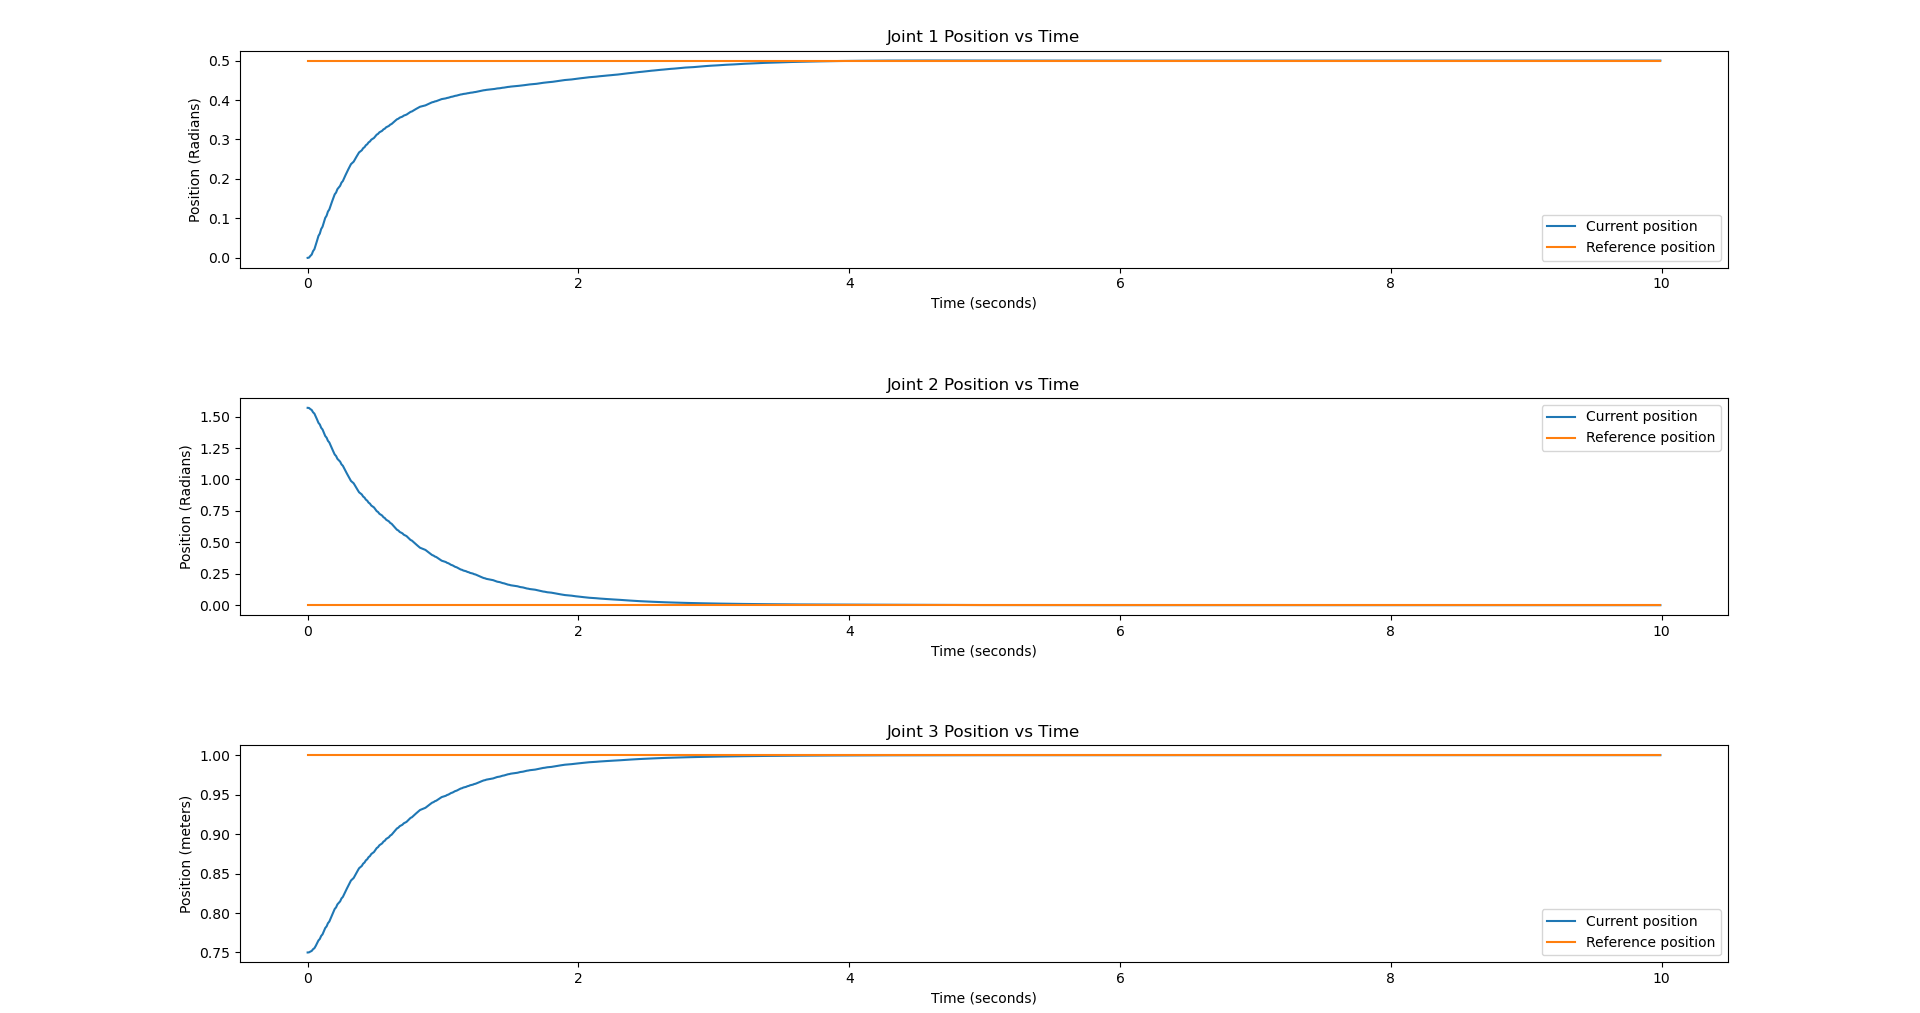
\includegraphics[width=8.5in, height=6.5in, center]{test_run_controller.png}
        \caption{An example set of plots that our graphing code generated, with all gains set to 10}
    \end{figure}
    The \lstinline{dump_graph_data} function is called every time that the 
    \lstinline{joint_states_callback} function is 
    called. This produces a significant amount of data, very quickly. Therefore, 
    we start this function with an `if' statement that will only run the following 
    code if it has been at least .01 seconds. We check to see if the iterator 
    variable is less than 1000, to ensure that the arrays end up having the same 
    dimensions for plotting. Once the joint value arrays have been filled to 
    maximum capacity, we then create a $3\times1$ subplot where each joint is plotted 
    against time.\\
    \vspace{0in}\\
    Later in the code, we reset both the joint value arrays and the iterator. 
    This allows us to enter a new reference position for the simulation to 
    achieve and the plotting will occur without having to entirely restart 
    the simulation.
\end{homeworkProblem}

\nobreak\extramarks{Problem 2}{}\nobreak{}

\begin{homeworkProblem}[Problem 2]
    \subsection{Tuning the PD Controller}
    
\end{homeworkProblem}

\end{document}